%
% File naacl2019.tex
%
%% Based on the style files for ACL 2018 and NAACL 2018, which were
%% Based on the style files for ACL-2015, with some improvements
%%  taken from the NAACL-2016 style
%% Based on the style files for ACL-2014, which were, in turn,
%% based on ACL-2013, ACL-2012, ACL-2011, ACL-2010, ACL-IJCNLP-2009,
%% EACL-2009, IJCNLP-2008...
%% Based on the style files for EACL 2006 by 
%%e.agirre@ehu.es or Sergi.Balari@uab.es
%% and that of ACL 08 by Joakim Nivre and Noah Smith

\documentclass[11pt,a4paper]{article}
\usepackage[hyperref]{naaclhlt2019}
\usepackage{times}
\usepackage{latexsym}

\usepackage{url}
\usepackage{times}  %Required
\usepackage{helvet}  %Required
\usepackage{courier}  %Required
\usepackage{url}  %Required
\usepackage{graphicx}  %Required


\usepackage{color}
\usepackage{mwe}
\usepackage{subfig}
\usepackage{amssymb}
\usepackage{mathtools}

\usepackage{latexsym}
\usepackage{multirow}
\usepackage[utf8]{inputenc}
\usepackage{dirtytalk}
\usepackage{multibib}
\usepackage{bm}
\usepackage{bbm}
\usepackage{amsmath}
\usepackage[linesnumbered,ruled]{algorithm2e}
\usepackage{amsfonts}
\usepackage{setspace}
\newcommand{\kechen}[1]{\textcolor{red}{[Kechen]: {#1}}}
\newcommand{\blue}[1]{\textcolor{green}{[Kechen]: {#1}}}
\newcommand{\cheng}[1]{\textcolor{red}{[Cheng]: {#1}}}
\newcommand{\softmax}{\textit{softmax}}
\newcommand{\maximize}{\textit{maximize}}

%\aclfinalcopy % Uncomment this line for the final submission
%\def\aclpaperid{123} %  Enter the acl Paper ID here

%\setlength\titlebox{5cm}
% You can expand the titlebox if you need extra space
% to show all the authors. Please do not make the titlebox
% smaller than 5cm (the original size); we will check this
% in the camera-ready version and ask you to change it back.

\newcommand\BibTeX{B{\sc ib}\TeX}

\title{Adapting RNN Sequence Prediction Model to Multi-label Set Prediction}

  
\author{Kechen Qin ~~~~ Cheng Li ~~~~ Virgil Pavlu ~~~~ Javed A. Aslam\\
  Khoury College of Computer Sciences \\
  Northeastern University\\
{\tt qin.ke@husky.neu.edu} ~~~~ {\tt \{chengli,vip,jaa\}@ccs.neu.edu}\\
   \\}

\date{}

\begin{document}
\maketitle
\begin{abstract}
We present an adaptation of RNN sequence models to the problem of multi-label classification for text, where the target is a \emph{set of labels}, not a sequence. Previous such RNN models define probabilities for sequences but not for sets; attempts to obtain a set probability are after-thoughts of the network design, including pre-specifying the label order, or relating the sequence probability to the set probability in \textit{ad hoc} ways.

Our formulation is derived from a principled notion of set probability, as the sum of probabilities of corresponding permutation \blue{permutation} sequences for the set. We provide a new training objective that maximizes this set probability, and a new prediction objective that finds the most probable set on test documents. These new objectives are theoretically appealing because they give the RNN model freedom to discover the best label order, which often is the natural one (but different among documents). 

We develop efficient procedures to tackle the computation difficulties involved in training and prediction. Experiments on benchmark datasets demonstrate that we outperform state-of-the-art methods for this task.

\end{abstract}

\section{Introduction}
\label{sec:Introduction}
% \kechen{alleviate exposure bias? related work}
Multi-label text classification is an important machine learning task wherein one must predict a set of labels to associate with a given document; for example, a news article might be tagged with labels \texttt{sport}, \texttt{football}, \texttt{2018 world cup}, and \texttt{Russia}. 
Formally, we are given a set
of label candidates $\mathcal{L}=\{1,2,...,L\}$,  and we aim to build a classifier 
which maps a document $x$ to a set of labels $\mathbf{y}\subset \mathcal{L}$. The label set $\mathbf{y}$ is typically written as a binary vector $\mathbf{y}\in \{0,1\}^L$, with each bit $y_{\ell}$
indicating the presence or absence of a label.

% A key research question in multi-label text classification is how to model and leverage the dependencies among labels.
Naively, one could predict each label independently without considering label dependencies. This approach is called Binary Relevance \cite{DBLP:journals/pr/BoutellLSB04,tsoumakas2007multi}, and is widely used  due to its simplicity, but it often does not deliver good performance.  Intuitively, knowing some labels---such as \texttt{sport} and \texttt{football}---should make it easier to predict \texttt{2018 world cup} and then \texttt{Russia}.  There are several methods that try to capture label dependencies by building a joint probability estimation over all labels  $p(\mathbf{y}=(y_1,y_2,...,y_L)|x)$ \cite{ghamrawi2005collective,read2009classifier,DBLP:conf/icml/DembczynskiCH10,li2016conditional}. 
% \kechen{put BR before the introduction of dependency? because there is nothing about dependency by using BR} 
The most popular approach, Probabilistic Classifier Chain (PCC) \cite{DBLP:conf/icml/DembczynskiCH10} learns and predicts labels one-by-one in a predefined fixed order: for each label, it uses one classifier to estimate the probability of that label given all previous labels predictions, $p(y_l|y_1,...,y_{l-1},x)$. PCC's well known drawback is that errors in early predictions tend to propagate to subsequent predictions, and can become massive when the total number of label candidates $L$ is large. 
% since PCC has to make a decision regarding each label candidate.






Recurrent neural networks (RNN) are originally designed to output a sequential structure, such as a sentence \cite{DBLP:conf/emnlp/ChoMGBBSB14}.  Recently, RNNs have also been applied to multi-label classification by mapping the label set to a sequence \cite{DBLP:conf/cvpr/WangYMHHX16,DBLP:journals/corr/ZhangWSZL16,DBLP:conf/icpr/JinN16,DBLP:conf/iccv/WangCLXL17,DBLP:journals/corr/abs-1709-08553,DBLP:conf/aaai/ChenCYW18,DBLP:journals/corr/abs-1806-04822}. In contrast to PCC where a binary decision is made for each label sequentially,  RNN only predicts the positive labels explicitly and therefore its decision chain length is equal to the number of positive labels, not the number of all labels.  Therefore RNN, while still suffers from early errors, propagates errors less than PCC. 

% Recurrent  neural networks (RNNs) are neural network models with recurrent structures. They are able to model dynamic temporal behaviors and are widely used in sequence modeling tasks such as machine translations.

% \begin{align}
% p(s_t=l|x) = [\softmax(\phi(f_t,h_t))]_l,
% \end{align}



%  RNN predictions \kechen{aka decoder} are typically done by maximizing the overall sequence probability, which is defined as $p(\mathbf{s}|x) = \prod_{t=1}^T p(s_t|x)$ \cheng{$\prod_{t=1}^T p(s_t|x,s_1,s_2,...,s_{t-1})$}.
% % \begin{align}
% % p(\mathbf{s}|x) = \prod_{t=1}^T p(s_t|x).
% % \label{eq:rnn_prob}
% % \end{align}
% The joint prediction is usually implemented approximately with a beam search.

% The input documents can be treated either as a sequence of words or a bag of words, and these words are represented by dense vectors.
% Attention mechanism proposed by \newcite{DBLP:journals/corr/BahdanauCB14}, at each timestep, selects important words associated with the prediction, and assign them high attention weights. After applying attention mechanism to the word representations, we can find corresponding words that are most related to the classification task and use them to predict the labels later. 

% Formally, feature words extracted by attention mechanism is called $f$, and are concatenated with hidden memory $h$ maintained by the RNN. The output vector will be passed through a nonlinearity $\phi$ before being sent to the output dense layer, and then output the probability attached with each label candidate. By multiplying over the probability of output label at each timestep $t$, the probability of the predicted label sequence can be represented as follows:



% where $[softmax()]_i$ is the $i$-th element in softmax output, and $s_t$ represents the predicted label at timestep $t$. 
% The whole pipeline is very similar to a machine translation, the model translate the document into a sequence of labels.

%Formally, the RNN and attention is built as follows:

%The model, grounded on gated recurrent units (GRU), consists of \textit{M} hidden layers, and at the \textit{k}th layer, the hidden state $h_t$ at timestep $t$ is derived as:

%\[ h_t^{(k)} = GRU(h_{t-1}^{(k)}, h_{t}^{(k-1)}) \]

%The output of the final hidden layer on the network is used as part of attention mechanism. This is similar to attention mechanism proposed by \newcite{DBLP:journals/corr/BahdanauCB14}:
 
% \[ e_{ij} = \phi_1(h_i, s_{j-1}) \]
% \[ \alpha_{ik} = \frac{exp(e_{ij})}{\sum_t exp(e_{ik})} \]
% \[ c_i = \sum_k \alpha_{ik}s_k \]

%where $\phi_1$ is a feedforward affine transforms followed by a nonlinearity. $c$ is the weighted sum of the word representation $s$. Then $c$ is concatenated with GRU output, and passed through another nonlinearity before being sent to the final softmax output layer. 

%The loss function is computed by summing up cross-entropy loss at each timestep $t$:

% \[ L(x,y) = -\sum_t logP(y_t|x,y<t)\]

Both PCC and RNN rely heavily on label orders in training and prediction. In multi-label data, the labels are given as sets, not necessarily with natural order.  RNN define a sequence probability (dynamically) while PCC define set probability (statically, sets are built in a predefined order). Various ways of arranging sets as sequences have been explored:  ordered alphabetically,  by frequency, based on a label hierarchy, or according to some label ranking algorithm \cite{liu2015optimality}. The experimental results show that which order to choose can have a significant impact on learning and prediction \cite{vinyals2015order,DBLP:conf/nips/NamMKF17,DBLP:conf/aaai/ChenCYW18}. In the above example, starting label predictions sequence with \texttt{Russia}, while correct, would make the other predictions very difficult.

Previous work has shown that it is possible to train an RNN on multi-label data without specifying the label order in advance. With special training objectives, RNNs can explore different label orders and converge to some order automatically \cite{vinyals2015order}. In this paper we follow the same line of study: We consider how to adapt RNN sequence model to multi-label set prediction without specifying the label order. Specifically, we make the following  contributions:
\begin{enumerate}
\item We analyze existing RNNs models proposed for multi-label prediction, and show that existing training and prediction objectives are not well justified mathematically and have undesired consequences in practice. 
% \item We are the first to make a clear distinction between sequence probability and set probability (in this learning setup), and treat set probability naturally as the sum of all corresponding sequence probabilities.
% \item Based on this set probability definition, we derive new training and prediction objectives that avoid the drawbacks of existing ones, and give the RNN model more freedom to automatically discover and utilize the best label orders.
\item  We develop efficient approximate training and prediction methods. We propose new training and prediction objectives based on a principled notion of set probability. Our new formulation avoids the drawbacks of existing ones and gives  the  RNN  model  freedom  to discover the best label order. 
\item We outperform state-of-the-art methods on several multi-label classification datasets.
\end{enumerate}
 % In this paper, we instead train RNNs by directly maximizing the probability of the \emph{label set}, which is defined as the sum of all sequence (set-permutations) probabilities---thus not constrained by a particular order.
 % % This approach gives the model the freedom to explore different orders in training and prediction and leads to better prediction performance. 
 % Our results on benchmark data sets demonstrate that our proposed method outperforms state-of-the-art methods for the task of multi-label set prediction.

\section{Mapping Sequences to Sets} 
In this section, we formulate how existing works map sequences to sets, by writing down their objective functions using consistent notations. To review RNN designed for sequences, let $\mathbf{s}=(s_1,s_2,...,s_T)$ be an input sequence of outcomes, in a particular order, where $T$ is the maximum number of labels in a document; the order is often critical to the datapoint. An RNN model defines a probability distribution over all possible output sequences given the input in the form $p(\mathbf{s}=(s_1,s_2,...,s_T)|x)=\prod_{t=1}^T p(s_t|x,s_1,s_2,...,s_{t-1})$. To train the RNN model, one maximizes the likelihood of the ground truth sequence $p(\mathbf{s}=(s_1,s_2,...,s_T)|x)$.

At prediction time, one seeks to find the sequence with the highest probability $\mathbf{s}^*=\arg\max_\mathbf{s} p(\mathbf{s}|x)$, and this is usually implemented approximately with a beam search procedure \cite{lowerre1976harpy} (we modified into Algorithm \ref{alg:beam_combine}). The sequence history is encoded with an internal memory vector $h_t$ which is updated over time. RNN is also often equipped with the attention mechanism \cite{DBLP:journals/corr/BahdanauCB14}, which in each timestep $t$ puts different weights on different words (features) and thus effectively attends on a list of important words. The context vector of selected words $c_t$ is computed as the weighted average over the dense representation of the words. The context $c_t$, the RNN memory $h_t$ at timestep $t$, and the previous label ${s_{t-1}}$ are concatenated and used to model the label probability distribution at time $t$ as $p(s_t|x,s_1,s_2,...,s_{t-1}) \sim  \softmax(\phi(c_t,h_t,s_{t-1}))$, where $\phi$ is a non-linear function, and $\softmax$ is the normalized exponential function generalizing binary logistic regression. %Other variants of RNN, such as sequence to sequence encoder-decoder structure \cite{DBLP:conf/emnlp/ChoMGBBSB14,DBLP:conf/nips/NamMKF17}, further take into account the word order in the documents. \kechen{remove last sentence?}


% \begin{algorithm}
%     \SetKwInOut{Input}{Input}
%     \SetKwInOut{Output}{Output}
%
%     % \underline{function Beam\_Search\_for\_Given\_Set} $(\mathbf{y},m)$\;
%     \Input{Instance $x$}
%     \Output{A list of top sequences and the associated probabilities}
%     Initialize $K$ empty sequences $\mathbf{s}_1$,$\mathbf{s}_2$,...,$\mathbf{s}_K$ \\
%     \While {not all $K$ sequences end with the STOP symbol}{
%         \For {each sequence $\mathbf{s}_k$}{
%         \eIf{sequence $\mathbf{s}_k$ does not end with the STOP symbol}{
%         \For {each label $\ell$ in $\mathcal{L}$}{
%         \If{sequence $\mathbf{s}_k$ does not contain $\ell$}{
%         generate new candidate sequence by combining $\mathbf{s}_k$ and $\ell$
%         }
%
%         }
%                 generate new candidate sequence by combining $\mathbf{s}_k$ and the STOP symbol\\}{
%         consider $\mathbf{s}_k$ itself as a candidate sequence
%         }
%
%
%             % $\mathbf{y}_t = \mathbf{y} - set(s_i)$ \\
%             % \For {$j=0;j<k_3;$}{
%             % \tcp{$l_j$ is the $j$-th most possible label inferred at timestep $t$}
%             %     \If{$l_j \in \mathbf{y}_t$}{
%             %         $s_{ij} \leftarrow s_i + l_j$\\
%             %         $j++$\\
%             %     }
%             % }
%         }
%
%     Select the top $K$ sequences among all candidates with the highest probability and assign them to $\mathbf{s}_1$,$\mathbf{s}_2$,...,$\mathbf{s}_K$
%         % \tcp{Prune sequence list to }
%         % $s \leftarrow s_{ij}[:k_3]$
%     }
%     \Return{sequence list $\mathbf{s}_1$,$\mathbf{s}_2$,...,$\mathbf{s}_K$ and the associated probabilities}
%     \caption{RNN\_Beam\_Search \cite{lowerre1976harpy}}
%     \label{alg:beam}
% \end{algorithm}



% combine beam
 % A typical multi-label dataset consists of $N$ training instances of the form $\{x^{(n)},\mathbf{y}^{(n)}\}$, where each $\mathbf{y}^{(n)}$ is an unordered set.
 
 
 \begin{table*}[t]
 	\begin{center}

\resizebox{1.03\textwidth}{!}{%
\hspace{-2ex}
 \begin{tabular}{|c|c|c|}
 \hline
 Methods	&Train objective	& Prediction\\
 \hline
 seq2seq-RNN & $\maximize \sum_{n=1}^N \log p(\mathbf{s}^{(n)}|x^{(n)})$ & $\hat{\mathbf{y}}=set(\mathbf{s}^*)$, $\mathbf{s}^*=\arg\max_{\mathbf{s}} p(\mathbf{s}|x)$\\
 \hline 
 Vinyals-RNN-max & $\maximize \sum_{n=1}^N \max_{\mathbf{s}\in \pi(\mathbf{y}^{(n)})}\log p(\mathbf{s}|x^{(n)})$ & $\hat{\mathbf{y}}=set(\mathbf{s}^*)$, $\mathbf{s}^*=\arg\max_{\mathbf{s}} p(\mathbf{s}|x)$\\
 \hline
 Vinyals-RNN-uniform & $\maximize \sum_{n=1}^N \sum_{\mathbf{s}\in \pi(\mathbf{y}^{(n)})}\log p(\mathbf{s}|x^{(n)})$ & $\hat{\mathbf{y}}=set(\mathbf{s}^*)$, $\mathbf{s}^*=\arg\max_{\mathbf{s}} p(\mathbf{s}|x)$\\
 \hline
 Vinyals-RNN-sample & $\maximize \sum_{n=1}^N \sum_{\mathbf{s}\in \pi(\mathbf{y}^{(n)})}p(\mathbf{s}|x^{(n)})\log p(\mathbf{s}|x^{(n)})$ & $\hat{\mathbf{y}}=set(\mathbf{s}^*)$, $\mathbf{s}^*=\arg\max_{\mathbf{s}} p(\mathbf{s}|x)$\\
 \hline
 set-RNN (ours) & $\maximize \sum_{n=1}^N \log \sum_{\mathbf{s}\in \pi(\mathbf{y}^{(n)})} p(\mathbf{s}|x^{(n)})$& $\hat{\mathbf{y}}=\arg\max_{\mathbf{y}} p(\mathbf{y}|x)$\\
 \hline
 \end{tabular}
 }
 \caption{Comparison between previous and our \emph{set-RNN} training and prediction objectives} \label{tab_objs}
 \end{center}
 \end{table*}
 
 
 To apply RNNs to multi-label problems, one has to map the given set of labels $\mathbf{y}$ to a sequence $\mathbf{s}=(s_1,s_2,...,s_T)$, on training documents. This is usually obtained by writing the label set in a globally fixed order (e.g.\ by label frequency), similar to PCC.
 % After mapping the ground truth set $\mathbf{y}^{(n)}$ to a sequence $\mathbf{s}^{(n)}$ with the chosen order for each training instance $(x^{(n)},\mathbf{y}^{(n)})$,
 Once mapping is done, RNN are trained with the standard maximum likelihood objective \cite{DBLP:conf/nips/NamMKF17}: 
\begin{align}
\maximize \sum_{n=1}^N \log p(\mathbf{s}^{(n)}|x^{(n)})
\label{eq:standard_rnn}
\end{align}
where $N$ is the total number of documents in the corpus. \newcite{vinyals2015order} proposes to dynamically choose during training the sequence order deemed as most probable by the current RNN model:
\begin{align}
\maximize \sum_{n=1}^N \max_{\mathbf{s}\in \pi(\mathbf{y}^{(n)})}\log p(\mathbf{s}|x^{(n)})
\label{eq:max_obj}
%\vspace{-2ex}
\end{align}
where the $\pi(\mathbf{y}^{(n)})$ stands for all  permutations of $\mathbf{y}^{(n)}$. This eliminates the need to manually specify label order.
However, as noticed by the authors, this objective cannot be used in the early training stages: the early order choice (often random) is reinforced by this objective and can be stuck upon permanently. To address this issue, \newcite{vinyals2015order}~also proposes two smoother alternative objectives to initialize the model training:

The authors suggest that one first consider many random orders for each label set in order to explore the space:
\begin{align}
\maximize \sum_{n=1}^N \sum_{\mathbf{s}\in \pi(\mathbf{y}^{(n)})}\log p(\mathbf{s}|x^{(n)})
\label{eq:wrong_obj}
\end{align} 

After that, one can sample sequences following the model predictive distribution instead of uniform distribution:
\begin{align}
\maximize \sum_{n=1}^N \sum_{\mathbf{s}\in \pi(\mathbf{y}^{(n)})}p(\mathbf{s}|x^{(n)})\log p(\mathbf{s}|x^{(n)})
\label{eq:sample_obj}
\end{align}  

In training, one needs to  schedule the transition among these objectives, a rather tricky endeavor. At prediction time, one needs to find the most probable set. This is done by (approximately) finding the most probable sequence $\mathbf{s}^*=\arg\max_\mathbf{s} p(\mathbf{s}|x)$ and treating it as a set $\hat{\mathbf{y}}=set(\mathbf{s}^*)$. With a large number of sequences, it is quite possible that the argmax has actually a low probability, which can lead to neglecting important information when we ignore sequences other than the top one.

% containing all labels in the sequence $s^*$ as the predicted set.




% These above existing techniques infer label sequentially, thus heavily depend on the input and output order. However, in practice, there is no way to know the global optimal label ordering prior to running the classification, so we have to use some approximations which might not reflect proper label dependency. In addition to that, imagine that when the model predict labels sequentially, a label in a fixed ordering can only learn the context ignoring long range dependencies and bidirectional dependencies. All these motivate us argue that text multi-label classification can be naturally expressed with sets rather than sequences, which means that predefined input and output orders are not necessary. We propose to treat input as bag of words instead of a sequence, and use random ordering to deliver the output. It not only significantly reduce the training time, but also saves the effort to search for the best label ordering. To further adopt the model in text multilabel classification, we design a two-level beam-search algorithm for generating the most possible label set attached with a document.



% \section{Related Work}
% \label{sec:RelatedWork}
% qkcqkc

%%%%%%%%%%%%%%%%%%%%%%%%%%%%%%%%%%%%%%%%%%%%%%%%%%%%%%%%%%%%%%%%%%%%%%%%%%%%%%%%

\section{Adapting RNN Sequence Prediction Model to Multi-label Set Prediction}
\label{sec:Model}

We propose a new way of adapting RNN to multi-label set prediction, which we call \emph{set-RNN}. We appreciate the RNN model structure \cite{rumelhart1988learning} (defines a probability distribution over all possible sequences directly) and introduce training and prediction objectives tailored for sets that take advantage of it, while making a clear distinction between the sequence probability $p(\mathbf{s}|x)$ and the set probability $p(\mathbf{y}|x)$. 
% We notice that previous work either lack an explicit definition of set probability, or use sequence probability as the set probability, or transform sequence probability into set probability in an ad hoc way. 
% We notice that while the idea of using RNN for multi-label prediction has a lot of advantages and potentials, the existing adaptations of RNN to set prediction task are not well justified and have several issues.
 % In the literature, these two are often used interchangeably.
 % A standard RNN model only defines a probability distribution over all possible sequences directly, as mentioned earlier.
  We define the set probability as the sum of sequences probabilities for all sequence permutations of the set, namely $p(\mathbf{y}|x)=\sum_{\mathbf{s}\in \pi(\mathbf{y})} p(\mathbf{s}|x)$. Based on this formulation, an RNN also defines a probability distribution over all possible sets indirectly since $\sum_{\mathbf{y}} p(\mathbf{y}|x)=\sum_{\mathbf{y}}\sum_{\mathbf{s}\in \pi(\mathbf{y})} p(\mathbf{s}|x)=\sum_{\mathbf{s}} p(\mathbf{s}|x)=1$.   
  % \kechen{It's still possible for the model to predict a label twice. I'd like to see a mathematical treatment of this case in your framework. Would you treat the predicted multiset as a set by ignoring repeated entries? Would you force the probability of a multiset down to zero? The mere fact that these can be predicted by the model means that they should eat away at some of the probability mass devoted to pure sets. You need a way of handling this. }
  To be precise, our label ``permutations'' $\pi$ are sequences that allow repetitions (i.e.\ $(y_1,y_2,y_3,y_1,...)$), up to a maximum length. So the set probability sums over all such permutations, and both training and prediction candidate sets are generated this way. In practice, we do not think this detail makes any difference, as sequences with repeated labels are extremely rare; however in theory we want to allow the attention context to focus on any recent labels it chooses to (repeated if necessary).
  
  
  In standard maximum likelihood training, one wishes to maximize the likelihood of given label sets, namely, $\prod_{n=1}^N p(\mathbf{y}^{(n)}|x^{(n)})=\prod_{n=1}^N \sum_{\mathbf{s}\in \pi(\mathbf{y}^{(n)})} p(\mathbf{s}|x^{(n)})$, or equivalently, 
\begin{align}
\maximize \sum_{n=1}^N \log \sum_{\mathbf{s}\in \pi(\mathbf{y}^{(n)})} p(\mathbf{s}|x^{(n)})
\label{eq:right_obj}
\end{align}
  % Having this clearly defined set probability is critical for our formulation as it naturally leads to our training and prediction methods.

% PCC... Recently, deep structured networks such as recurrent (RNN) neural networks have become increasingly popular in multi-label classification domain. Especially, it shows a great success in image multi-label classification. On the other hand, for text data, due to RNNs' ability to capture input dependency, they can be used to both encode words into a document representation, and then decode the document representation into labels sequentially. This is the so-called encoder-decoder structure\cite{DBLP:conf/emnlp/ChoMGBBSB14}. \newcite{DBLP:conf/nips/NamMKF17} apply encoder-decoders on text multilabel classification. Their experimental results show that the encoder-decoders can achieve very good performance on low cardinality text dataset by ordering the positive labels using frequency.

% \subsection{Proposed Method}


\subsection{How is our new formulation different?}

This training objective (\ref{eq:right_obj}) looks similar to the objective (\ref{eq:wrong_obj}) considered in previous work \cite{vinyals2015order}, but in fact they correspond to very different transformations. Under the maximum likelihood framework, our objective (\ref{eq:right_obj}) corresponds to the transformation $p(\mathbf{y}|x)=\sum_{\mathbf{s}\in \pi(\mathbf{y})} p(\mathbf{s}|x)$, while objective (\ref{eq:wrong_obj}) corresponds to the transformation $p(\mathbf{y}|x)=\prod_{\mathbf{s}\in \pi(\mathbf{y})} p(\mathbf{s}|x)$. The latter transformation does not define a valid probability distribution over $\mathbf{y}$ (i.e., $\sum_{\mathbf{y}} p(\mathbf{y}|x)\neq 1$), and it has an undesired  consequence in practical model training: because of the multiplication operation, the RNN model has to assign equally high probabilities to all sequence permutations of the given label set in order to maximize the set probability. 
Using Jensen’s inequality, one can show that the total probability mass in Eq. 3 will be less than or equal to the true amount of probability mass in Eq. 1. In this sense, previous work is optimizing a bound on the log-likelihood, while we are optimizing it directly. 

If only some sequence permutations receive high probabilities while others receive low probabilities, the set probability will still be low in Eq. 3. In other words, if for each document, RNN finds one  good way of ordering relevant labels (such as hierarchically) and allocates most of the probability mass to the sequence in that order, the model will be penalized heavily.  As a consequence the model has little freedom in discovering and concentrating on some natural label order. In contrast, with our proposed training objective, in which the multiplication operation is replaced by the  summation operation, it suffices to find only one reasonable permutation of the labels for each document. \emph{Different documents can have different label orders}; thus our proposed training objective gives the RNN model far more freedom on label order. The other two objectives (\ref{eq:max_obj}) and (\ref{eq:sample_obj}) proposed in \cite{vinyals2015order} are less restrictive than  (\ref{eq:wrong_obj}), but they have to work in conjunction with (\ref{eq:wrong_obj}) because of the self reinforcement issue. Our proposed training objective has a natural probabilistic interpretation, does not suffer from self reinforcement issue and can serve as a stand alone training objective. 
% Another approach used in previous work, which is to pick one fixed sequence order (e.g., by label frequency) in advance, forces the model to only assign high probabilities to sequences in that order.
% , and therefore does not leave any opportunity for the model to explore label orders. Since in multi-label data, labels often do not have an obvious ordering and human heuristics are often suboptimal, it is advantageous to let the training procedure discover label orderings, on a per sample basis.
% \subsection{A Brief Review of RNN and Attention}

\begin{algorithm}
    \SetKwInOut{Input}{Input}
    \SetKwInOut{Output}{Output}

    % \underline{function Beam\_Search\_for\_Given\_Set} $(\mathbf{y},m)$\;
    \Input{Instance $x$ \\
    Subset of labels considered $G\subset \mathcal{L}$\\
    Boolean flag $ALL$: 1 if sequences must contain all $G$ labels; 0 if partial sequences are allowed }
    \Output{A list of top sequences and the associated probabilities} 
    Let $\mathbf{s}_1$,$\mathbf{s}_2$,...,$\mathbf{s}_K$ be the top $K$ sequences  found so far. Initially, all $K$ sequences are empty. $\oplus$ means concatenation. \\
    % Let $C$ be the set of candidate sequences, initially empty.\\
    \While {true}{
     // Step 1: Generate Candidate Sequences from each existing sequence $s_k \in K$ and all possible new labels $l \in G\setminus s_k$:\\
    Expand all non-stopped sequences:\\
     % $C = \{ \mathbf{s}_k\oplus l | l\in G,  l \notin s_k, STOP \notin s_k \}$\\
     $C = \{ \mathbf{s}_k\oplus l | l\in G, STOP \notin s_k \}$\\    
Include stopped sequences:\\
    $C = C \cup \{ \mathbf{s}_k | STOP \in s_k \}$\\
    Terminate non-stopped sequences:\\
    \If{$ALL==0$}{
    % Add $\mathbf{s}_k\oplus STOP$ to $C$  }
    %
    $C =C \cup \{ \mathbf{s}_k\oplus STOP | STOP \notin s_k \}$
    }


    %         \For {each sequence $\mathbf{s}_k$ that does not end with $STOP$}{
    % Add to $C$ all possible new candidate sequences in the form $\mathbf{s}_k\oplus l$, where $l$ is a label in $G$ but not in $\mathbf{s}_k$, and $\oplus$ stands for concatenation.\\
    % \If{CONTAIN\_ALL=FALSE}{Add $\mathbf{s}_k\oplus STOP$ to $C$  }
    % }
    % \For {each sequence $\mathbf{s}_k$ that ends with $STOP$}{
    % Add $\mathbf{s}_k$  to $C$
    % }

 // Step 2: Select highest probabilities sequences from candidate set $C$\\
    % From the candidate set $C$ generated by all $\mathbf{s}_k$ in Step 1, select the top $K$ candidates with the highest probabilities and use them as new values for $\mathbf{s}_1$,$\mathbf{s}_2$,...,$\mathbf{s}_K$\\
    $K$
    % = \{$\mathbf{s}_1$,$\mathbf{s}_2$,...,$\mathbf{s}_K$\}
    =  topK-argmax$_k \{\text{prob}[s_k] | s_k \in C\}$\\
    \If {all top $K$ sequences end with $STOP$ or contain all labels in $G$}{
    Terminate the algorithm}

        % \tcp{Prune sequence list to }
        % $s \leftarrow s_{ij}[:k_3]$
     }
    \Return{sequence list $\mathbf{s}_1$,$\mathbf{s}_2$,...,$\mathbf{s}_K$ and the associated probabilities}
    \caption{Beam\_Search}
    \label{alg:beam_combine}
\end{algorithm}

\subsection{Training by Maximizing Set Probability}
Training an RNN model with the proposed objective (\ref{eq:right_obj}) requires summing up sequence (permutation) probabilities for a set $\mathbf{y}$, where $|\mathbf{y}|$ is the cardinality of the set. Thus evaluating this objective exactly can be intractable. We can approximate this sum by only considering the top $K$ high probability sequences produced by the RNN model. We introduce a variant of beam search for sets with width $K$ and with the search candidates in each step restricted to only labels in the set (see Algorithm~\ref{alg:beam_combine}). This approximate inference procedure is carried out repeatedly before each batch training step, in order to find high probability sequences for all training instances occurring in that batch. The overall training procedure is summarized in Algorithm \ref{alg:train_beam}.% \cheng{add pseudo code}

\begin{algorithm}
    \SetKwInOut{Input}{Input}
    \SetKwInOut{Output}{Output}

  %  \underline{function Euclid} $(a,b)$\;
    \Input{Multi-label dataset $(x^{(n)},\mathbf{y}^{(n)}),n=1,2,...,N$ }
    \Output{Trained RNN model parameters}
    
    % Initialize model parameters\\
    \ForEach {batch}{
        % \ForEach {batch }{
            \ForEach{$(x^{n},\mathbf{y}^{n})$ in the batch}{
                Get top $K$ sequences :\\
		    	$\{\mathbf{s}^n_{1},...,\mathbf{s}^n_{K}, p(\mathbf{s}^n_{1}|x^n),...,p(\mathbf{s}^n_{K}|x^n)\}$=  \hspace{4ex}=Beam\_Search($(x^{n},\mathbf{y}^{n}, ALL=1$)\\
                }
            Update model parameters by maximizing $\sum\limits_{(x^{n},\mathbf{y}^{n}) \in \text{batch}} \log \sum\limits_{\mathbf{s}\in\{\mathbf{s}^n_{1},...,\mathbf{s}^n_{K}\}} p(\mathbf{s}|x^{n})$
        % }
    }
    \caption{Training method for set-RNN}
    \label{alg:train_beam}
\end{algorithm}


\subsection{Predicting the Most Probable Set}
The transformation $p(\mathbf{y}|x)=\sum_{\mathbf{s}\in \pi(\mathbf{y})} p(\mathbf{s}|x)$ also naturally leads to a prediction procedure, which is different from the previous standard of directly using most probable sequence as a set. We instead aim to find the most likely set $\hat{\mathbf{y}}=\arg\max_{\mathbf{y}} p(\mathbf{y}|x)$, which involves summing up probabilities for all of its permutations (see Table~1). To make it tractable, we propose a two-level beam search procedure. First we run standard RNN beam search (Algorithm \ref{alg:beam_combine}) to generate a list of high probability sequences.  We then consider the label set associated with each label sequence.  For each set, we evaluate its probability using the same approximate summation procedure as the one used during model training (Algorithm~\ref{alg:beam_combine}): we run our modified beam search to find the top few high probability sequences associated with the set and sum up their probabilities. Among these sets that we have evaluated, we choose the one with the highest probability as the prediction. The overall prediction procedure is summarized in Algorithm~\ref{alg:test}. As we shall show in case study, the most probable set may not correspond to the most probable sequence; these are certainly cases where our method has an advantage.
%\textbf{Variant of beam search.} To obtain the top high probability sequences associated with a given set, beam search


Both our method and the comparison sate-of-the-art RNN takes more time than a vanilla-RNN, by a factor of $K$, because there are $K$ permutations for each datapoint. Our proposed method is slower than the RNN baseline by a factor of 1.5 (approximatively) because each epoch requires one more forward pass. 

% \begin{algorithm}
%     \SetKwInOut{Input}{Input}
%     \SetKwInOut{Output}{Output}
%
%     % \underline{function Beam\_Search\_for\_Given\_Set} $(\mathbf{y},m)$\;
%     \Input{Instance $x$ and a set of labels $\mathbf{y}$ }
%     \Output{A list of top sequence permutations for the given label set and the associated probabilities}
%     Initialize $K$ empty sequences $\mathbf{s}_1$,$\mathbf{s}_2$,...,$\mathbf{s}_K$ \\
%     \For {$t=0;\ t<len(\mathbf{y});\ t++\ $}{
%         \For {each sequence $\mathbf{s}_k$ and each label $\ell$ in $\mathbf{y}$}{
%         \If{sequence $\mathbf{s}_k$ does not contain $\ell$}{
%         generate new candidate sequence by combining $\mathbf{s}_k$ and $\ell$\\
%         }
%
%             % $\mathbf{y}_t = \mathbf{y} - set(s_i)$ \\
%             % \For {$j=0;j<k_3;$}{
%             % \tcp{$l_j$ is the $j$-th most possible label inferred at time stamp $t$}
%             %     \If{$l_j \in \mathbf{y}_t$}{
%             %         $s_{ij} \leftarrow s_i + l_j$\\
%             %         $j++$\\
%             %     }
%             % }
%         }
%     Select the top $K$ sequences among all candidates with the highest probability and assign them to $\mathbf{s}_1$,$\mathbf{s}_2$,...,$\mathbf{s}_K$
%         % \tcp{Prune sequence list to }
%         % $s \leftarrow s_{ij}[:k_3]$
%     }
%     \Return{sequence list $\mathbf{s}_1$,$\mathbf{s}_2$,...,$\mathbf{s}_K$ and the associated probabilities}
%     \caption{Beam\_Search\_for\_Given\_Set}
%     \label{alg:beam_predict}
% \end{algorithm}


\begin{algorithm}
    \SetKwInOut{Input}{Input}
    \SetKwInOut{Output}{Output}

 %   \underline{function Euclid} $(a,b)$\;
    \Input{Instance $x$}
    \Output{Predicted label set $\hat{\mathbf{y}}$}
    Obtain $K$ highest probability sequences :\\
    $\{\mathbf{s}_1,...,\mathbf{s}_{K}\}$ =  Beam\_Search((x,$\mathcal{L}, ALL=0$)\\
    
    Map each sequence $\mathbf{s}_k$ to the corresponding set $\mathbf{y}_k$ and remove duplicate sets (if any)
    
    \ForEach {$\mathbf{y}_k$}{
        % $\hat{\mathbf{y_i}} \leftarrow set(\mathbf{s_i})$\\
        
         Get $K$ most probable sequences associated with $\mathbf{y}_k$ and their probabilities :\\
	   $\{\mathbf{s'}_{1},...,\mathbf{s'}_{K}, p(\mathbf{s}'_{1}|x),...,p(\mathbf{s}'_{K}|x)\}$= \\ \hspace{6ex} =Beam\_Search((x,$\mathbf{y}_k, ALL=1$)\\
       Set probability is approx by summing up :
        $p({\mathbf{y}_k}|x) \approx \sum\limits_{\mathbf{s}\in \{\mathbf{s}'_{1},...,\mathbf{s}'_K\}} p(\mathbf{s}|x)$
    }    
    $\hat{\mathbf{y}} = argmax_{{\mathbf{y}_k}}(p({\mathbf{y}_k}|x))$
    \caption{Prediction Method for Set-RNN}
    \label{alg:test}
\end{algorithm}


%Recurrent neural network (RNN) is a class of neural network models. The key point that makes RNN different from a standard feedforward neural network model is that it contains a recurrent structure and . In this work, we first represent a text as bags of words, and pre-trained the word representation $s$ by using  word2vec\cite{DBLP:journals/corr/abs-1301-3781}. We use gated recurrent units with \textit{M} hidden layers. At the bottom layer, we feed the pre-trained label representations to the RNN, and at the \textit{k}th RNN layer, the hidden state $h_j$ is derived as:

% \[ h_k^{(t)} = GRU(h_{t-1}^{(k)}, h_{t}^{(k-1)}) \]

%  The final hidden layer on the network also take the encoded representation \textit{c} as context using an attention mechanism. 
 
%  \[ h_k^{(t)} = RELU(GRU(h_{t-1}^{(k)}, h_{t}^{(k-1)}); c) \]
 
%  Context vector \textit{c} is the weighted sum of the word representation $s$. This is similar to attention mechanism proposed by \newcite{DBLP:journals/corr/BahdanauCB14}:
 
%  \[ e_{ij} = \phi(h_i, s_{j-1}) \]
%  \[ \alpha_{ik} = \frac{exp(e_{ij})}{\sum_t exp(e_{ik})} \]
%  \[ c_i = \sum_k \alpha_{ik}s_k \]

% where $\phi$ is a feedforward affine transforms followed by a \textit{tanh} nonlinearity.



\section{Results and Analysis}
\label{sec:results}
\subsection{Experimental Setup}

We test our proposed set-RNN method on 4 real-world datasets, RCV1-v2, Slashdot, TheGuardian, and Arxiv Academic Paper Dataset (AAPD) \cite{DBLP:journals/corr/abs-1806-04822}. We take the public RCV1-v2 release\footnote{\scriptsize\url{http://www.ai.mit.edu/projects/jmlr/papers/volume5/lewis04a/lyrl2004_rcv1v2_README.htm}} and randomly sample 50,000 documents. We crawl Slashdot and TheGuardian documents from their websites\footnote{\scriptsize Slashdot: \url{https://slashdot.org/} Note that there is another public Slashdot multi-label dataset \cite{read2009classifier} but we do not use that one because it is quite small. TheGuardian: \url{https://www.theguardian.com}  
} and treat the official editor tags as ground truth. We also gather a list of user tags\footnote{\scriptsize \url{www.zubiaga.org/datasets/socialbm0311/}} for each document and treat them as additional features. For AAPD dataset, we follow the same train/test split as in \cite{DBLP:journals/corr/abs-1806-04822}. Table \ref{tab:stats} contains statistics of these four datasets. 
\begin{table}[h]
	\resizebox{1.01\columnwidth}{!}{%resize the table
\begin{tabular}{|l|c|c|c|c|c|c|}
  \hline
  Data & \#Train & \#Test & Cardinality & \#Labels & Doc length  \\
  \hline
  Slashdot & 19,258 & 4,814& 4.15& 291&64 \\
  RCV1-v2 & 40,000& 10,000&  3.17& 101&121 \\
  TheGuardian & 37,638 & 9,409 & 7.41& 1,527&505 \\
  AAPD & 53,840 & 1,000 & 2.41& 54 & 163 \\
  \hline
\end{tabular}
}
\caption{\fontsize{10}{12}\selectfont  Statistics of the datasets.}\label{tab:stats}
\end{table}


\begin{table*}[ht]
	\begin{center}
	\resizebox{2.1\columnwidth}{!}{%resize the table
		\begin{tabular}{|l|cc|cc|cc|cccc|}
			\hline
			\multirow{2}{*}{Methods}	&  
             \multicolumn{2}{c|}{Slashdot}&\multicolumn{2}{c|}{RCV1-v2}&\multicolumn{2}{c|}{TheGuardian}&\multicolumn{4}{c|}{AAPD} \\
             \cline{2-11}
           & label-F1 & instance-F1  & label-F1 & instance-F1 & label-F1 & instance-F1 & label-F1 & instance-F1 & Hamming-Loss & Micro-F1 \\

                        \hline
            BR
            & .271 & .484 & .486 & .802 &.292 & .572 & .529 & .654 & .0230 & .685 \\
            BR-support
            & .247 & .516 & .486 & .805 &.296 & .594 & .545 & .689 & \textbf{.0228} & .696\\
            PCC 
            & .279 & .480 & .595 & .818 &- & - & .541 & .688 & .0255 & .682 \\
            seq2seq-RNN  
             & .270 & .528 & .561 & .824 &.331 & .603 & .510 & .708 & .0254 & .701 \\
            Vinyals-RNN-uniform 
             & .279 & .527 & .578 & .826 & .313 & .567  & .532 & .721 & .0241 & .711\\
            Vinyals-RNN-sample
            & .300 & .531 & .590 & .828 & .339 & .597 & .527 & .706 & .0259 & .697 \\
            Vinyals-RNN-max
            & .293 & .530 & .588 & .829 & .343 & .599 & .535 & .709 & .0256 & .700 \\
            Vinyals-RNN-max-direct
             & .226 & .518 & .539 & .808 & .313 & .583 & .490 & .702 & .0257 & .694\\
            SGM
            &-&-&-&-&-&-& - & - & .0245 & .710 \\
            set-RNN 
             & \textbf{.310} & \textbf{.538} & \textbf{.607} & \textbf{.838}  &\textbf{.361} & \textbf{.607} & \textbf{.548} & \textbf{.731} & .0241 & \textbf{.720}\\
            \hline

		\end{tabular}
		}
	\end{center}
	\caption{Comparison of different approaches. ``-'' means result not available. For \emph{hamming loss}, the lower the value is, the better the model performs. For all other measures, the higher the better.%\kechen{cardinality analysis, V's method can't perform well on Guardian. why?}
    }\label{tab:main}
\end{table*}





\begin{table*}[ht]
  \begin{center}
  	\resizebox{2.1\columnwidth}{!}{%resize the table

    \begin{tabular}{|l|cc|cc|cc|cc|}
      \hline
      \multirow{2}{*}{Methods}  &  
             \multicolumn{2}{c|}{Slashdot}&\multicolumn{2}{c|}{RCV1-v2}&\multicolumn{2}{c|}{TheGuardian}&\multicolumn{2}{c|}{AAPD} \\
             \cline{2-9}
           & label-F1 & instance-F1  & label-F1 & instance-F1 & label-F1 & instance-F1 & label-F1 & instance-F1\\

                        \hline
            seq2seq-RNN  
             & .270$\to$.269 & .528$\to$.528& .561$\to$.561 & .824$\to$.824 &.331$\to$.336& .603$\to$.603 & .510$\to$.511 &.708$\to$.709 \\
            Vinyals-RNN-uniform  
             & .279$\to$.288& \textbf{.527}$\to$\textbf{.537}& .578$\to$.587& .826$\to$.833& \textbf{.313}$\to$\textbf{.336}& \textbf{.567}$\to$\textbf{.585} & \textbf{.532}$\to$\textbf{.542} &.721$\to$.724 \\
             Vinyals-RNN-sample
            & .300$\to$.303 & .531$\to$.537 &.590$\to$.597 & .828$\to$.833 & \textbf{.339}$\to$\textbf{.351} & .597$\to$.602 & .527$\to$.530 & .706$\to$.708 \\
            Vinyals-RNN-max
            & .293$\to$.301 & .530$\to$.535 & .588$\to$.585 & .829$\to$.830 & .343$\to$.352 &.599$\to$.604 & .535$\to$.537 &.709$\to$.712  \\
            Vinyals-RNN-max-direct
             & .226$\to$.228& .518$\to$.519& .539$\to$.538& .808$\to$.808& .313$\to$.316&.583$\to$.584 & .490$\to$.490 &.702$\to$.701 \\
            
            set-RNN 
             & \textbf{.297}$\to$\textbf{.310} & \textbf{.528}$\to$\textbf{.538} & \textbf{.593}$\to$\textbf{.607} & .831$\to$.838 &\textbf{.349}$\to$\textbf{.361} & \textbf{.595}$\to$\textbf{.607} & .548$\to$.548 &.728$\to$.731 \\\hline

    \end{tabular}
    }
  \end{center}
  \caption{Predicting the most probable sequence vs. predicting the most probable set. Numbers before the arrow: predicting the most probable sequence. Numbers after the arrow: predicting the most probable set. We highlight scores which get significantly improved in \textbf{bold} (improvement is larger than 0.01).
    }\label{table_prediction}
\end{table*}

 To process documents, we filter out stopwords and punctuations. Each document is truncated to have maximum 500 words for TheGuardian and AAPD, and 120 for Slashdot and RCV1-v2. Numbers and out-of-vocabulary words are replaced with special tokens. Words, user tags and labels are all encoded as 300-dimensional vectors using \textsc{word2vec} \cite{DBLP:journals/corr/abs-1301-3781}.
 
 We implement RNNs with attention using \textsc{tensorflow-1.4.0} \cite{DBLP:conf/osdi/AbadiBCCDDDGIIK16}. The dynamic function for  RNNs is chosen to be Gated recurrent units (GRU) with  2 layers and at most 50 units in decoder. The  size of the GRU unit is 300. We set dropout rate to 0.3, and train the model with Adam optimizer \cite{DBLP:journals/corr/KingmaB14} with learning rate $0.0005$. Beam size is set to be 12 at both training and inference stages. We adopt \emph{label-F1} (average F1 over labels) and \emph{instance-F1} (average F1 over instances) as our main evaluation metrics, as defined below:
 
\begin{align*} \text{label-F1} = \frac{1}{L}\sum_{\ell=1}^L\frac{2\sum_{n=1}^N y^{(n)}_\ell \hat{y}^{(n)}_\ell}{\sum_{n=1}^N y^{(n)}_\ell+\sum_{n=1}^N \hat{y}^{(n)}_\ell}\\
\text{instance-F1} = \frac{1}{N}\sum_{n=1}^N\frac{2\sum_{\ell=1}^L y^{(n)}_\ell \hat{y}^{(n)}_\ell}{\sum_{\ell=1}^L y^{(n)}_\ell+\sum_{\ell=1}^L \hat{y}^{(n)}_\ell}
\end{align*}
where for each instance $n$, $y_\ell^{(n)}=1$ if label $\ell$ is a given label in ground truth; $\hat{y}_\ell^{(n)}=1$ if label $\ell$ is a predicted  label.

We compare our method with the following methods: 
\begin{itemize}
	\item \textbf{Binary Relevance (BR)} \cite{tsoumakas2007multi} with both independent training and prediction;
	\item \textbf{Binary Relevance with support inference (BR-support)} \cite{wang2017regularizing} which trains binary classifiers independently but imposes label constraints at prediction time by only considering label sets observed during training, namely $\hat{\mathbf{y}}=\arg\max_{\text{observed~}\mathbf{y}}\prod_{\ell=1}^L p(y_{\ell}|x)$;
	\item \textbf{Probabilistic Classifier Chain (PCC)} \cite{DBLP:conf/icml/DembczynskiCH10} which transforms the multi-label classification task into a chain of binary classification problems.
    \item \textbf{Sequence to Sequence RNN (seq2seq-RNN)} \cite{DBLP:conf/nips/NamMKF17} which maps each set to a sequence by decreasing label frequency and solves the multi-label task with an RNN designed for sequence prediction (see Table \ref{tab_objs}). 
    \item \textbf{Vinyals-RNN-uniform, Vinyals-RNN-sample, and Vinyals-RNN-max} are three variants of RNNs proposed by \cite{vinyals2015order}. They are trained  with different objectives that correspond to different transformations between sets and sequences. See Table~\ref{tab_objs} for a summary of their training objectives. Following the approach taken by \cite{vinyals2015order}, Vinyals-RNN-sample and Vinyals-RNN-max are initialized by Vinyals-RNN-uniform. We have also tested training Vinyals-RNN-max directly without having Vinyals-RNN-uniform as an initialization, and we name it as  \textbf{Vinyals-RNN-max-direct}.
    \item \textbf{Sequence Generation Model (SGM)} \cite{DBLP:journals/corr/abs-1806-04822} which trains the RNN model similar to seq2seq-RNN but uses a new decoder structure that computes a weighted global embedding based on all labels as opposed to just the top one at each time step.
\end{itemize}

In BR and PCC, logistic regressions with L1 and L2 regularizations are used as the underlying binary classifiers. seq2seq-RNN, PCC, and SGM rely on a particular label order. We adopt the decreasing label frequency order, which is the most popular choice.

%Additionally in order to measure the effect of summing up sequence probabilities at prediction time, we test a variant of seq2seq RNN (named seq2seq RNN w/ set pred) which sums up sequence probabilities during prediction, and a variant of our proposed method (named set-RNN w/o set pred) which only predicts the most probable sequence.

% For fixed ordering experiments, we keep the order of both input and output, which means we are using a sequence-to-sequence (seq2seq) \cite{DBLP:conf/nips/SutskeverVL14}. To be specific, we represent the document as a sequence of words, then sort the output labels based on count of occurrences in descending order. This setup is the same as \newcite{DBLP:conf/nips/NamMKF17}'s work,  that's why we call it \textsc{fix\_order\_Nam}. For non fixed ordering experiments, in contrary to ordered sequences, we represent the document as a bag of words and feed the labels into the model as a set. We set beam width 12 and 6 in two-level beam search, which means we select top 12 sequences based on sequence probability and rerank them with their set probability based on top 6 permutations. We name our model \textsc{blabla}.

% \textbf{Results.}

\subsection{Experimental Results}
% \kechen{split this section into subsections?}

% \kechen{I have a slight concern about the scalability of this approach, both with varying beam size and number of labels. I'm curious about the computational complexities of the training and prediction methods provided in the Algorithm 2 and Algorithm 3 and how that compares with existing methods.}

Table \ref{tab:main} shows the performance of different methods in terms of \emph{label-F1} and \emph{instance-F1}. The SGM results are taken directly from \cite{DBLP:journals/corr/abs-1806-04822}, and are originally reported only on AAPD dataset in terms of Hamming-Loss and Micro-F1. Definitions of these two metrics can be found in \cite{koyejo2015consistent}.  
% The second best method is the variant of our method without the sequence probability summation at prediction. Comparing these two, we can see the benefit of summing up sequence probabilities at prediction time (the beam search for summation step does not add much computation). 

 
Our method performs the best in all metrics on all datasets (except hamming loss on AAPD, see table \ref{tab:main}). In general, RNN based methods perform better than traditional methods BR, BR-support and PCC. Among the Vinyals-RNN variants, Vinyals-RNN-max and Vinyals-sample work the best and have similar performance. However, they have to be initialized by Vinyals-RNN-uniform. Otherwise, the training gets stuck in early stage and the performance degrades significantly. One can see the clear degradation by comparing the Vinyals-RNN-max row (with initialization) with the Vinyals-RNN-max-direct row (without initialization). By contrast, our training objective in set-RNN does not suffer from this issue and can serve as a stable stand alone training objective.

\begin{figure}[t]
%\hspace{-2ex}
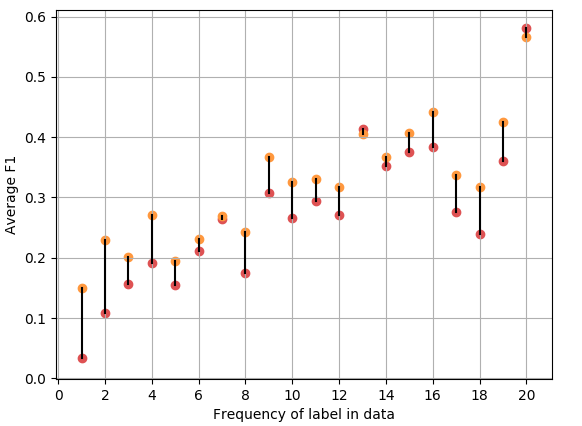
\includegraphics[width=1.0\columnwidth]{figs/labelf1.png}

\caption{Average F1 over rare labels with the same frequency on TheGuardian dataset. Orange=set-RNN, Red=seq2seq-RNN.}
\label{fig:labelf1}
%\vspace{-6ex}
\end{figure}

On TheGuardian dataset, set-RNN performs slightly better than seq2seq-RNN in terms of instance-F1, but much better in terms of label-F1. It is known that instance-F1 is basically determined by the popular labels' performance while label-F1 is also sensitive to the performance on rare labels. Figure~\ref{fig:labelf1} shows that set-RNN predicts rare labels better than seq2seq-RNN.

Next we analyze how much benefit our new set prediction strategy brings in. For each RNN-based method, we test two prediction strategies: 1) finding the sequence with the highest probability and outputting the corresponding set (this is the default prediction strategy for all models except set-RNN); 2) outputting the set with the highest approximated probability (this is the default prediction strategy for set-RNN). Table~\ref{table_prediction} shows how each method performs with these two prediction strategies. One can see that Vinyals-RNN-uniform and set-RNN benefit most from predicting the top set,  Vinyals-RNN-sample, Vinyals-RNN-max and Vinyals-RNN-max-direct benefit less, and seq2seq RNN does not benefit at all. Intuitively, for the top-set prediction to be different from the top-sequence prediction, the model has to spread probability mass across different sequence permutations of the same set. 

\subsection{Analysis: Sequence Probability Dsitribution}
Results in Table~\ref{table_prediction} motivates us to check how sharply (or uniformly) distributed the probabilities are over different sequence permutations of the predicted set. We first normalize these sequence probabilities related to the predicted set and then compute the entropy. To make predictions with different set sizes (and hence different number of sequence permutations) comparable, we further divide the entropy by the logarithm of number of sequences. Smaller entropy values indicate a sharper distributions. The results are shown in Figure~\ref{fig:entropy}.

seq2seq-RNN trained with fixed label order and standard RNN objective (\ref{eq:standard_rnn}) generates very sharp sequence distributions. It basically only assigns probability to one sequence in the given order. The entropy is close to 0. In this case, predicting the set is no different than predicting the top sequence (see Table~\ref{table_prediction}). On the other extreme is Vinyals-RNN-uniform, trained with objective (\ref{eq:wrong_obj}), which spreads probabilities across many sequences, and leads to the highest entropy among all models tested (the uniform distribution has the max entropy of 1). From Table~\ref{table_prediction}, we see that by summing up sequence probabilities and predicting the most probable set,  Vinyals-RNN-uniform's performance  improves. But as  discussed earlier, training with the objective (\ref{eq:wrong_obj}) makes it impossible for the model to discover and concentrate on a particular natural label order (represented by a sequence). Overall Vinyals-RNN-uniform is not competitive even with the set-prediction enhancement. Between the above two extremes are Vinyals-RNN-max and set-RNN (we have omitted Vinyals-RNN-sample and Vinyals-RNN-max-direct here as they are similar to Vinyals-RNN-max). Both models are allowed to assign probability mass to a subset of sequences. Vinyals-RNN-max produces sharper sequence distributions than set-RNN, because  Vinyals-RNN-max has the incentive to allocate most of the probability mass to the most probable sequence due to the max operator in its training objective (\ref{eq:max_obj}). From Table~\ref{table_prediction}, one can see that set-RNN clearly benefits from summing up sequence probabilities and predicting the most probable set while Vinyals-RNN-max does not benefit much. Therefore, the sequence probability summation is best used in both training and prediction, as in our proposed method.

Comparing 4 datasets in Table~\ref{table_prediction}, we also see that Slashdot and TheGuardian, which have larger label cardinalities (therefore more permutations for one set potentially), benefit more from predicting the most probable set than RCV1 and AAPD, which have smaller label cardinalities.

% By design, Vinyals-RNN-uniform and set-RNN could spread probabilities mass across many sequence permutations of the same set, Vinyals-RNN-sample, Vinyals-RNN-max and Vinyals-RNN-max-direct tends to allocate most of the probability mass to the top sequence, and seq2seq basically only assigns probability to the sequence in the given order. 

% To further validate our intuition, 


% seq2seq-RNN performs better than traditional methods BR, BR w/support and PCC. Adding set probability summation at prediction time does not further improve its performance. We suspect that since the model is trained to respect the given label order (decreasing label frequency order in this case), at prediction time, only sequences (roughly) in that order receives decent probabilities. Therefore the set probability is basically determined by the top sequence. Thus the sequence probability summation is best used in both training and prediction, as in our proposed method.


% (1) We can see that Vinyal\_final performs much better than Vinyal\_final\_noinit, which shows evidence to support our hypothesis that objective \ref{eq:max_obj} have to be initialized by a model pretrained with objective \ref{eq:wrong_obj}. Compare Vinyal- 

% (2) Vinyal\_final outperforms seq2seq RNN in Slashdot and RCV-v2, but not in TheGuardian. When cardinality is large, Vinyal's method can easily get stuck on bad prediction (and reinforce it). Comparing with Vinyal's method, our method is more stable and performs well in all three data sets.

% (3) Adding set prediction helps in both Vinyal's and our methods. \kechen{(1) difference between sample and max (2) labelF1 and InstanceF1 (3) highlight in table 4.}

\begin{figure}[t]
%\hspace{-2ex}
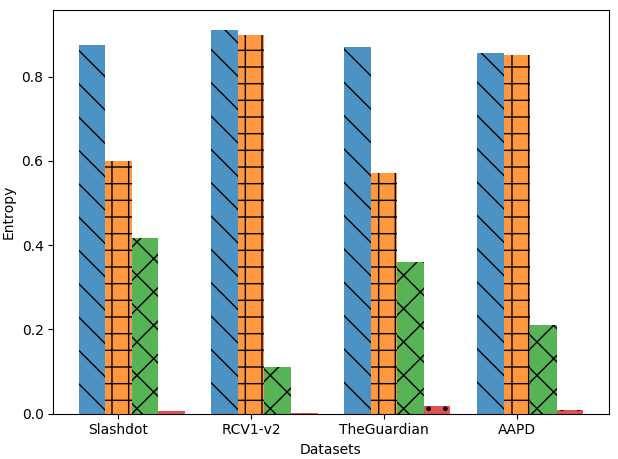
\includegraphics[width=1.00\columnwidth]{figs/entropy.png}

\caption{Entropy of sequence probability distribution for each model. Blue(\textbackslash)=Vinyals-RNN-uniform, Orange(+)=set-RNN, Green($\times$)=Vinyals-RNN-max, Red($\cdot$)=seq2seq-RNN.}
\label{fig:entropy}
%\vspace{-6ex}
\end{figure}


% \textbf{Entropy Analysis} We normalize the probabilities of top probable sequences inferred via different decoding algorithms, and compute entropy of the normalized probability distribution. The experimental result shows how different methods, which correspond to different objectives, generate different shapes of sequence distribution. The smaller entropy indicates sharper sequence probability distribution.

% (1) Training with standard RNN objective (objective \ref{eq:standard_rnn}) generates very sharp sequence probability distribution. 

% (2) Similar to RNN objective, Vinyal\_final (objective \ref{eq:max_obj}) maximizes the probability of the top sequence prediction, with additional ability to train on changing top prediction. This is why it is less sharper than RNN. The model assign the top sequence prediction a large probability, while probabilities of other predictions are very small.

% (3) Vinyal\_init is trying to optimize product of sequence probability (objective \ref{eq:wrong_obj}). Having avoided negative influence from exceptionally small probability, the model assign these predictions relatively uniform probabilities (the biggest entropy).

% (4) The entropy of our method (objective \ref{eq:right_obj}) is in the middle between vinit and vfinal. It demonstrates that our model assign relatively large probability to multiple sequences.




  % \begin{figure*}[ht]

  % \begin{minipage}{.5\linewidth}
  % \centering
  % \subfloat[]{\label{main:a}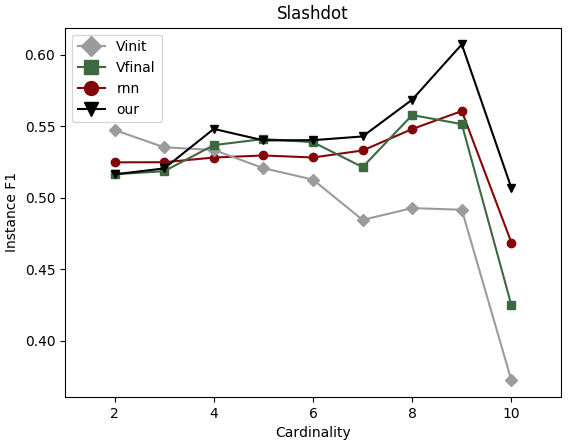
\includegraphics[scale=.35]{figs/slash.png}}
  % \end{minipage}%
  % \begin{minipage}{.5\linewidth}
  % \centering
  % \subfloat[]{\label{main:b}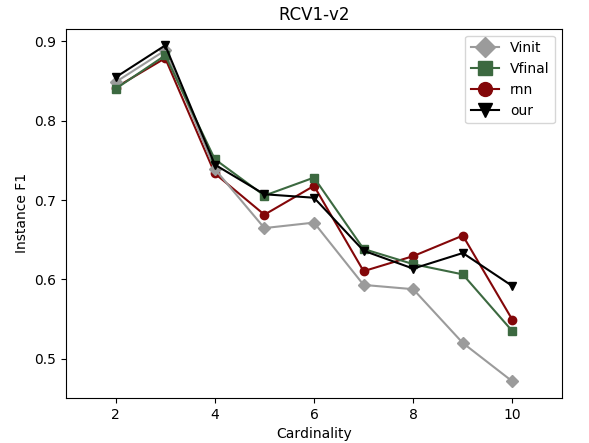
\includegraphics[scale=.35]{figs/reuter.png}}
  % \end{minipage}\par\medskip
  % \centering
  % \subfloat[]{\label{main:c}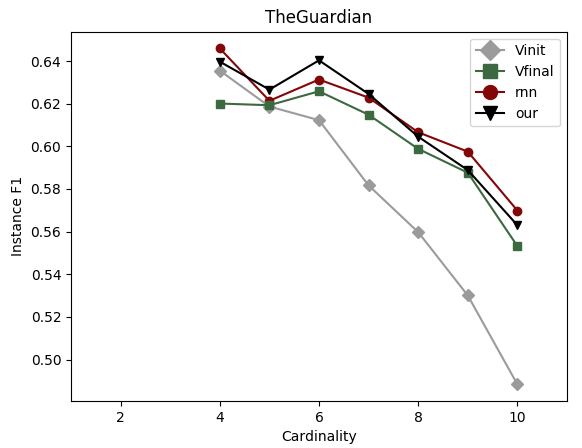
\includegraphics[scale=.35]{figs/guardian.png}}

  % \caption{Performance of different models on different cardinality subset}
  % \label{fig:main}
  % \end{figure*}


% \textbf{Cardinality Analysis} We group documents with the same cardinality into different subsets and individually present instance F1 on each subset. 

% (1) The performance of Vinyal\_init drops a lot as the cardinality increases.

% (2) The performance of our method scales well with cardinality. It outperforms other methods when cardiality is large.

% (3) 
\section{Case Analysis}
We further demonstrate how set-RNN works with two examples.
In the first example from the RCV1-v2 dataset, the most probable set predicted by set-RNN (which is also the correct set in this example) does not come from the most probable sequence. Top sequences in decreasing probability order are listed in Table~\ref{tab:pred_case_study}. The correct label set \{forex, markets, equity, money markets, metals trading, commodity\} has the maximum total probability of 0.161, but does not match the top sequence.

% \small{
% \texttt{ \footnotesize{ \linespread{0.1}
% FOCUS-Dollar romps, weak Dow blunts share rallies. The dollar romped ahead against the mark on Tuesday and European bourses also prospered, with British blue chips breaking records, but share rallies were blunted by a weaker Wall Street start.The dollar sneaked above the psychological 1.50 marks barrier in early European trade. It continued to firm as the day progressed and a wave of fund buying propelled its towards 1.51."Once we moved beyond 1.50, it\'s momentum-driven," said Keld Holm, international economist at Lehman BrothersIt is now trading above levels seen on July 16, when dollar/mark suffered its biggest one-day drop this year as New York share prices crashed.The dollar also rallied to 1.2345 Swiss francs -- up sharply from its 1.2157 close in Europe on MondayThe dollar rally began on Monday after Bundesbank council member Ernst Welteke said there was room for further German interest rate cuts if M3 money supply growth continued to slow....
% His comment knocked the mark across the board and the dollar was further spurred overnight by Wall Street\'s strong Monday performance and a jump in Treasuries.On the bourses, leading shares in London, Frankfurt and Paris all got an early leg-up by the overnight surge on the Dow, which posted its biggest one-day gain in over a month to close 1.3 percent up.Im morning trading Tuesday London\'s blue-chip FTSE 100 index jumped more than 20 points to a record 3,933.6, surpassing its previous record of 3,922.1 set on August 28. However, after a weaker start on Wall Street Tuesday, it fell back sharply to close just below its record closing high at 3,916.1, up just 5.3 points. Analysts said London\'s gains had also been held in check by a lacklustre performance by government bonds, overshadowed by worries that Britain will cut interest rates further to stoke pre-election growth regardless of the inflation risk.In Frankfurt, German shares ended a lively floor trade session higher, with the 30-share DAX index closing at 2,570.95 points, up 22.22. In later electronic trading German shares fell back slightly under the influence of New York but dealers said the ever strengthening dollar (which would make German goods cheaper for foreigners) and firm government bonds were continuing to provide support.The same motors, plus gains in the French franc, propelled Paris shares, which started firmer and quickly strengthened. However, the main CAC-40 index fell back after Wall Street\'s York\'s shaky start to finish just off the day\'s high, up 21.82 points or 1.08 percent at 2,042.12.Stock and currency markets remained gripped by interest rate prospects following last Friday\'s U.S. jobs data showing lower unemployment and stronger earnings.U.S. producer and consumer price data -- due Thursday and Friday -- will be scrutinized for fresh signs of inflation pressures. Many traders and investors are betting on a rise of 0.25 percentage point in U.S. interest rates when the Federal Open Market Committee next meets on September 24.Opinions are mixed as to whether the central bank will decide this time to raise or leave interest rates unchanged, perhaps until after the November 5 presidential election.CURRENCIES AT 1600 GMTThe dollar was at 1.5088 marks and 109.85 yen compared with late European levels on Monday of 1.4935 and 109.15.STOCK MARKETSThe Financial Times-Stock Exchange index of 100 leading British shares closed up 5.3 points at 3,916.1.In Paris, the CAC-40 share index closed up 21.82 at 2,042.12.The 30-share DAX index in Frankfurt closed up 22.22 at 2,570.95.PRECIOUS METALSGold closed unchanged from Monday\'s close at 383.45. Silver finished at \$5.11, up two cents.'
% }
% }



% bag of words set:
% \texttt{ \footnotesize{ \linespread{0.1}
% foreign, monday, blu, begin, govern, data, shaky, surpass, live, sneak, pari, econom, clos, support, point, pre, im, french, trad, rate, barry, treasur, leav, low, dollar, council, unemploy, metal, britain, produc, show, meet, job, street, weltek, inflat, strong, swiss, propel, knock, percent, earn, firm, germ, romp, wall, progress, decid, dax, anal, frankfurt, suff, cent, franc, year, cut, brother, prec, sign, continu, grip, novemb, overnight, bundesbank, spur, open, move, index, level, growth, silf, fts, lacklustr, gmt, strength, record, bet, lead, floor, time, mark, keld, electron, prospect, stock, prosp, gain, presid, cac, motor, ernst, remain, commit, held, thursday, perform, sharp, july, compar, memb, fresh, elect, good, pric, overshadow, break, buy, morn, early, bours, septemb, stok, back, opinion, rise, pressur, post, lehm, deal, european, start, due, risk, exchang, comment, scrutin, focus, session, month, worry, big, late, chip, tuesday, cheap, unchang, m3, slight, psych, feder, interest, dow, europ, set, suppl, drop, jump, fund, market, rais, wav, room, weak, financ, momentum, board, brit, mix, leg, driv, high, consum, main, prev, finish, intern, york, make, check, slow, bond, holm, currenc, quick, day, crash, london, ahead, yen, money, bank, end, fell, august, invest, friday, influ, gold, provid, surg, shar, rally, blunt
% }
% }


\begin{table}[h]
\resizebox{1.01\columnwidth}{!}{%resize the table
\begin{tabular}{l|l}
PROB	& SEQUENCE\\
\hline
0.0236 	& equity, markets, money markets, forex\\
0.0196	& {\bf forex, markets, equity, money markets, metals trading, commodity}\\
0.0194	& {\bf equity, markets, forex, money markets, metals trading, commodity}\\
0.0159	& {\bf markets, equity, forex, money markets, metals trading, commodity}\\
0.0157	& {\bf forex, money markets, equity, metals trading, markets, commodity}\\
0.0153	& {\bf forex, money markets, markets, equity, metals trading, commodity}\\
0.0148	& markets, equity, money markets, forex\\
0.0143	& {\bf money markets, equity, metals trading, commodity, forex, markets}\\
0.0123	& {\bf markets, money markets, equity, metals trading, commodity, forex}\\
0.0110 	& {\bf markets, equity, forex, money markets, commodity, metals trading}\\
0.0107	& {\bf forex, markets, equity, money markets, commodity, metals trading}\\
0.0094	& {\bf forex, money markets, equity, markets, metals trading, commodity}\\
\hline
\end{tabular}
}
\caption{The set-RNN predicted set (also the correct set) \{forex, markets, equity, money markets, metals trading, commodity\} has the max total probability of 0.161, but does not match the top sequence. Sequences for the correct set are in bold.}\label{tab:pred_case_study}
\end{table}

%%%%%%%%%%%%%%%%%%%%%%%%%%%%%%%%%%%%%%%%%%%%%%%%%%%%%%%%%%%%%%%%%%%%%%%%%%%%%%%%
%%%%%%%%%%%%%%%%%%%%%%%%%%%%%%%%%%%%%%%%%%%%%%%%%%%%%%%%%%%%%%%%%%%%%%%%%%%%%%%%
Next we demonstrate the issue with prescribing the sequence order in seq2seq-RNN with a TheGuardian example\footnote{\scriptsize This document can be viewed at \url{http://www.guardian.co.uk/artanddesign/jonathanjonesblog/2009/apr/08/altermodernism-nicolas-bourriaud}}. Figure~\ref{fig:models} shows the predictions made by seq2seq-RNN and our method. In this particular example the top sequence agrees with the top set in our method's prediction so we can just analyze the top sequence. seq2seq-RNN predicts \texttt{Tate Modern} (incorrect but more popular label) while we predict \texttt{Tate Britain} (correct but less popular label). The seq2seq predicted sequence is in the decreasing label frequency order while our predicted sequence is not. In the training data, \texttt{Exhibition} is more frequent than \texttt{Tate Britain} and \texttt{Tate Modern}. If we arrange labels by decreasing frequency, \texttt{Exhibition} is immediately followed by \texttt{Tate Modern} 19 times, and by \texttt{Tate Britain} only 3 times. So it is far more likely to have \texttt{Tate Modern} than \texttt{Tate Britain} after \texttt{Exhibition}. However, at the set level, \texttt{Exhibition} and \texttt{Tate Modern} co-occurs 22 times while \texttt{Exhibition} and \texttt{Tate Britain} co-occurs 12 times, so the difference is not so dramatic. In this case, imposing the sequence order biases the probability estimation and leads to incorrect predictions.
%
% In the second case analysis present a case analysis document to show how the set-model is superior to the sequence-model for multilabel text classification. Ground Truth Label (sorted by frequency): ‘Culture’ ‘Art and Design’ ‘Art’ ‘Exhibitions’ ‘Tate Britain’. Extracted keywords by attention (over all steps): Tate, Curators, Newspapers, Exhibition, Philosophers, Art, Britain, Science, Doctor, Journalistic, Reviews, Artwork, Delta, Avant, Fashion, Literature, Grade, Manifesto.
%
%
% Top word evidences extracted by attention show that keywords are good enough for text multilabel prediction task (from this example, we show that ground truth labels can be inferred by these keywords). We don’t have to encode the documents as a sequence. We can use bag of words to represent the document.
% In Figure~\ref{fig:models} $h$ is the hidden history state. $h_0$ is the initial hidden state, which is randomly initialized by the model. $SOS$ is the start of the sentence symbol and $EOS$ is the end of the sentence symbol.
% In the training set, Frequency of bigram (exhibition, tate modern)=19, Frequency of bigram (exhibition, tate british)=3
% ``Tate modern'' is associated with exhibition, and ``tate britain'' is associated with ``painting and art''
% So it is very likely to predict tate modern after exhibition, if we sort the labels by frequency. 
% Our set prediction method can learn the optimal order and then make predictions. It is easy to predict ``tate britain'' given label ``art'' as history and top evidences extracted by attention mechanism.

% Set prob of culture art and design art exhibition tate modern = 0.095
% Set prob of the other one = 0.07
% \begin{figure}[h]
% 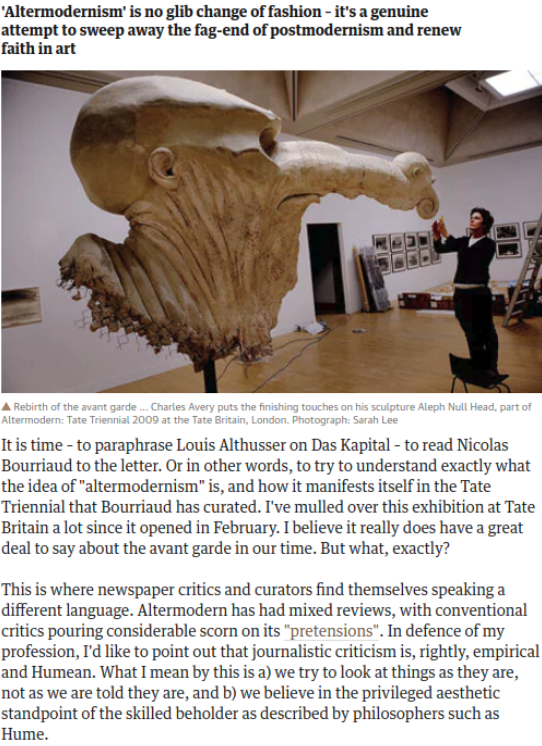
\includegraphics[width=\columnwidth]{figs/docexample.png}
% \caption{\fontsize{10}{12}\selectfont Example document (text shown incomplete). Ground Truth Label (sorted by frequency): ‘Culture’ ‘Art and Design’ ‘Art’ ‘Exhibitions’ ‘Tate Britain’.\\
% Extracted keywords by attention (over all steps): Tate, Curators, Newspapers, Exhibition, Philosophers, Art, Britain, Science, Doctor, Journalistic, Reviews, Artwork, Delta, Avant, Fashion, Literature, Grade, Manifesto.}
% \label{fig:example}
% \end{figure}
% \begin{figure}[t]
% \hspace{-2ex}
% 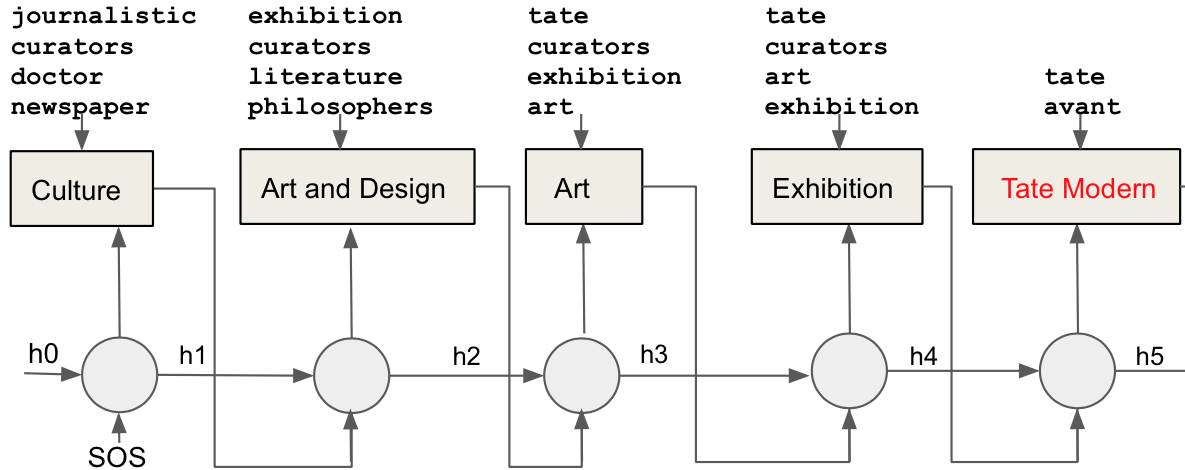
\includegraphics[width=1.2\columnwidth]{figs/train_sequence.png}
%
% \label{fig:models}
% \end{figure}
\begin{figure}[t]
%\hspace{-2ex}
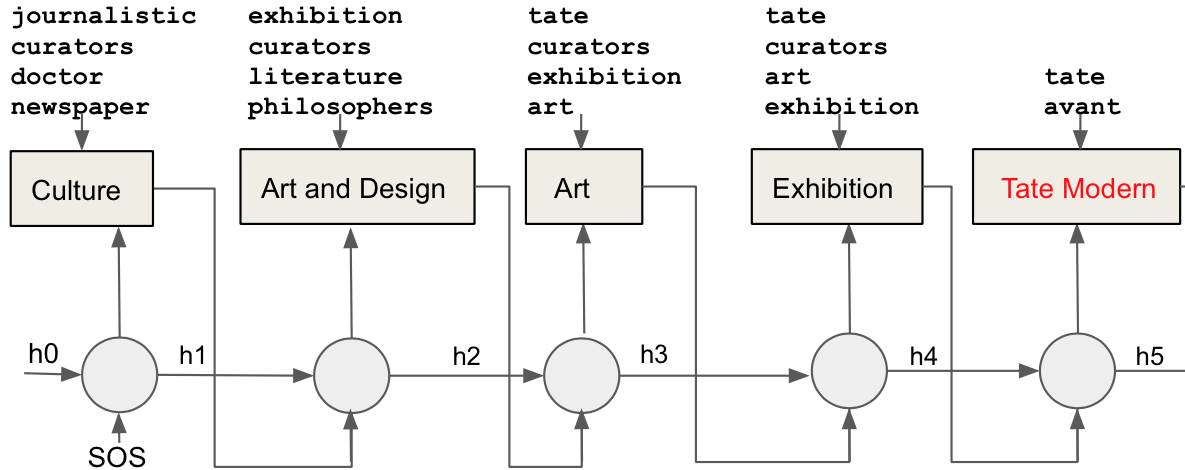
\includegraphics[width=1.0\columnwidth]{figs/train_sequence.png}
%\vspace{-4ex}
%\hspace{-2ex}
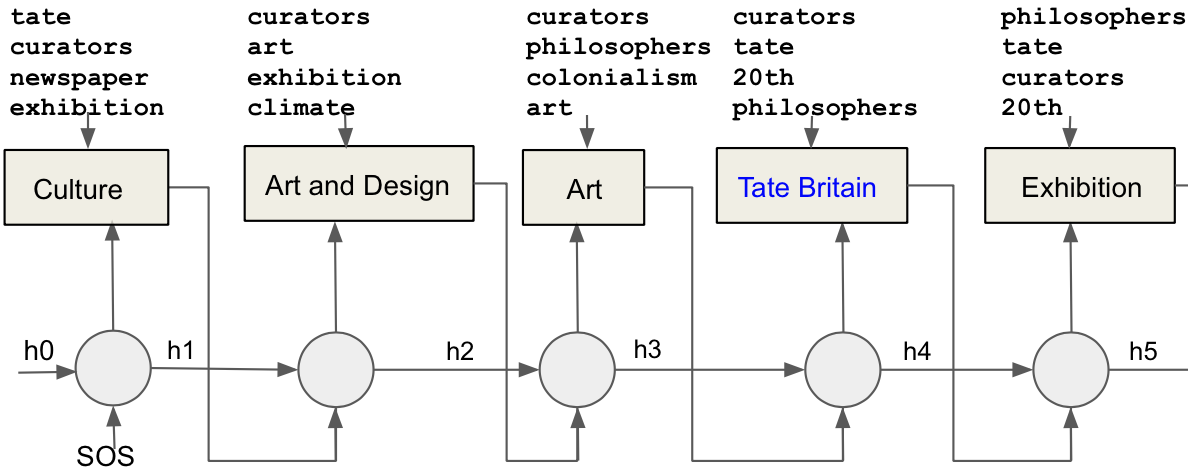
\includegraphics[width=1.0\columnwidth]{figs/train_set.png}

\caption{\fontsize{10}{12}\selectfont Top: best sequence by seq2seq-RNN; bottom: best sequence by set-RNN. Above models, at each time, we list the top unigrams selected by attention.\vspace{2ex}}
\label{fig:models}
%\vspace{-6ex}
\end{figure}
\section{Conclusion}
In this work, we present an adaptation of RNN sequence models to the problem of multi-label classification for text. RNN only directly defines probabilities for sequences, but not for sets. Different from previous approaches, which either transform a set to a sequence in some pre-specified order, or relate the sequence probability to the set probability in some ad hoc way, our formulation is derived from a principled notion of set probability. We define the set probability as the sum of all corresponding sequence permutation probabilities. We derive a new training objective that maximizes the set probability and a new prediction objective that finds the most probable set. These new objectives are theoretically more appealing than existing ones, because they give the RNN model more freedom to automatically discover and utilize the best label orders.
 % We develop efficient procedures to tackle the computations difficulties involved in training and prediction. Experiments on benchmark data sets demonstrate that our method outperforms state-of-the-art methods for this task, especially on rare labels.

\label{sec:conclusion}

\section{Acknowledgements}
We thank reviewers for their helpful comments, 
Krzysztof Dembczyński for his suggestions on comparisons, and
Xiaofeng Yang for help on writing. This work
has been generously supported through a grant from the
Massachusetts General Physicians Organization.
% \section{backup}
% \label{sec:backup}
%             seq2seq-RNN  
             & 0.270$\to$0.269 & 0.528$\to$0.528& 0.561$\to$0.561 & 0.824$\to$0.824 &\textbf{0.331}$\to$\textbf{0.336}& 0.603$\to$0.603\\
            Vinyals-RNN-uniform  
             & \textbf{0.279}$\to$\textbf{0.288}& \textbf{0.527}$\to$\textbf{0.537}& \textbf{0.578}$\to$\textbf{0.587}& \textbf{0.826}$\to$\textbf{0.833}& \textbf{0.313}$\to$\textbf{0.336}& \textbf{0.567}$\to$\textbf{0.585}\\
             Vinyals-RNN-sample
            & \textbf{0.300}$\to$\textbf{0.303} & \textbf{0.531}$\to$\textbf{0.537} & \textbf{0.590}$\to$\textbf{0.597} & \textbf{0.828}$\to$\textbf{0.833} & \textbf{0.339}$\to$\textbf{0.351} & \textbf{0.597}$\to$\textbf{0.602} \\
            Vinyals-RNN-max
            & \textbf{0.293}$\to$\textbf{0.301} & \textbf{0.530}$\to$\textbf{0.535} & 0.588$\to$0.585 & \textbf{0.829}$\to$\textbf{0.830} & \textbf{0.343}$\to$\textbf{0.352} & \textbf{0.599}$\to$\textbf{0.604} \\
            Vinyals-RNN-max-direct
             & \textbf{0.226}$\to$\textbf{0.228}& \textbf{0.518}$\to$\textbf{0.519}& 0.539$\to$0.538& 0.808$\to$0.808& \textbf{0.313}$\to$\textbf{0.316}& \textbf{0.583}$\to$\textbf{0.584}\\
             

\begin{table*}[ht]
	\begin{center}
		\begin{tabular}{|l|cc|cc|cc|}
			\hline
			\multirow{2}{*}{Methods}	&  
             \multicolumn{2}{c|}{Slashdot}&\multicolumn{2}{c|}{RCV1-v2}&\multicolumn{2}{c|}{TheGuardian} \\
             \cline{2-7}
           & label-F1 & instance-F1  & label-F1 & instance-F1 & label-F1 & instance-F1\\

                        \hline

            BR
            & 0.271 & 0.484 & 0.486 & 0.802 &0.292 & 0.572 \\
            BR-support
            & 0.247 & 0.516 & 0.486 & 0.805 &0.296 & 0.594 \\
            PCC 
            & 0.279 & 0.480 & 0.595 & 0.818 &- & - \\
            seq2seq-RNN  
             & 0.270 & 0.528 & 0.561 & 0.824 &0.331 & 0.603 \\
            Vinyals-RNN-uniform 
             & 0.279 & 0.527 & 0.578 & 0.826 & 0.313 & 0.567 \\
            Vinyals-RNN-sample
            & 0.300 & 0.531 & 0.590 & 0.828 & 0.339 & 0.597 \\
                        Vinyals-RNN-max
            & 0.293 & 0.530 & 0.588 & 0.829 & 0.343 & 0.599 \\
            Vinyals-RNN-max-direct
             & 0.226 & 0.518 & 0.539 & 0.808 & 0.313 & 0.583 \\
            set-RNN 
             & \textbf{0.310} & \textbf{0.538} & \textbf{0.607} & \textbf{0.838}  &\textbf{0.361} & \textbf{0.607} \\
            \hline

		\end{tabular}
        \newline
        \vspace*{0.1 cm}
        \newline
		\begin{tabular}{|l|cccc|}
			\hline
			\multirow{2}{*}{Methods}	&  
             \multicolumn{4}{c|}{AAPD} \\
             \cline{2-5}
           & label-F1 & instance-F1 & Hamming-Loss & Micro-F1 \\

                        \hline

            BR
            & - & - & 0.0316 & 0.646  \\
            PCC 
            & - & - & 0.0306 & 0.651 \\
            seq2seq-RNN  
             & 0.510 & 0.708 & 0.0254 & 0.701 \\
            Vinyals-RNN-uniform 
             & 0.532 & 0.721 & 0.0241 & 0.711 \\
            Vinyals-RNN-max
            & 0.535 & 0.709 & 0.0256 & 0.700 \\
            SGM
            & - & - & 0.0245 & 0.710 \\
            set-RNN 
             & \textbf{0.548} & \textbf{0.731} & \textbf{0.0241} & \textbf{0.720} \\
            \hline

		\end{tabular}
	\end{center}
	\caption{Comparison of different approaches. PCC experiment could not finish on TheGuardian dataset. For \emph{hamming loss}, the lower the value is, the better the model performs. %\kechen{cardinality analysis, V's method can't perform well on Guardian. why?}
    }\label{tab:main}
\end{table*}





\begin{table*}[ht]
  \begin{center}
    \begin{tabular}{|l|cc|cc|cc|}
      \hline
      \multirow{2}{*}{Methods}  &  
             \multicolumn{2}{c|}{Slashdot}&\multicolumn{2}{c|}{RCV1-v2}&\multicolumn{2}{c|}{TheGuardian} \\
             \cline{2-7}
           & label-F1 & instance-F1  & label-F1 & instance-F1 & label-F1 & instance-F1\\

                        \hline

 %           \textsc{PCC\_ensemble}  
 %           &0.0 & 0.0 & 0.0 & 0.0 & 0.0 & 0.0 \\


            seq2seq-RNN  
             & 0.270$\to$0.269 & 0.528$\to$0.528& 0.561$\to$0.561 & 0.824$\to$0.824 &\textbf{0.331}$\to$\textbf{0.336}& 0.603$\to$0.603\\
            Vinyals-RNN-uniform  
             & \textbf{0.279}$\to$\textbf{0.288}& \textbf{0.527}$\to$\textbf{0.537$\ast$}& \textbf{0.578}$\to$\textbf{0.587}& \textbf{0.826}$\to$\textbf{0.833}& \textbf{0.313}$\to$\textbf{0.336$\ast$}& \textbf{0.567}$\to$\textbf{0.585$\ast$}\\
             Vinyals-RNN-sample
            & \textbf{0.300}$\to$\textbf{0.303} & \textbf{0.531}$\to$\textbf{0.537} & \textbf{0.590}$\to$\textbf{0.597} & \textbf{0.828}$\to$\textbf{0.833} & \textbf{0.339}$\to$\textbf{0.351$\ast$} & \textbf{0.597}$\to$\textbf{0.602} \\
            Vinyals-RNN-max
            & \textbf{0.293}$\to$\textbf{0.301} & \textbf{0.530}$\to$\textbf{0.535} & 0.588$\to$0.585 & \textbf{0.829}$\to$\textbf{0.830} & \textbf{0.343}$\to$\textbf{0.352} & \textbf{0.599}$\to$\textbf{0.604} \\
            Vinyals-RNN-max-direct
             & \textbf{0.226}$\to$\textbf{0.228}& \textbf{0.518}$\to$\textbf{0.519}& 0.539$\to$0.538& 0.808$\to$0.808& \textbf{0.313}$\to$\textbf{0.316}& \textbf{0.583}$\to$\textbf{0.584}\\
            
            set-RNN 
             & \textbf{0.297}$\to$\textbf{0.310$\ast$} & \textbf{0.528}$\to$\textbf{0.538$\ast$} & \textbf{0.593}$\to$\textbf{0.607$\ast$} & \textbf{0.831}$\to$\textbf{0.838} &\textbf{0.349}$\to$\textbf{0.361$\ast$} & \textbf{0.595}$\to$\textbf{0.607$\ast$}\\\hline

    \end{tabular}
  \end{center}
  \caption{Predicting the most probable sequence vs predicting the most probable set. Numbers before the arrow: predicting the most probable sequence. Numbers after the arrow: predicting the most probable set. \kechen{We highlight scores which get improved in \textbf{bold}, and with $\ast$ ().}
    }\label{table_prediction}
\end{table*}

\clearpage
\newpage

\bibliography{local,naaclhlt2019}
\bibliographystyle{acl_natbib}

\appendix


\end{document}
